\documentclass{template/socthesis}

\usepackage[czech]{babel}
\usepackage[T1]{fontenc} % evropské uvozovky
\usepackage{csquotes}
\usepackage{xpatch}
\usepackage[author=,status=draft]{fixme} % vkládání poznámek  
% dva módy (status): draft (poznámky se zobrazují v PDF) / final (poznámky se nezobrazují v PDF)

\usepackage{subcaption}
\usepackage[backend=biber,bibstyle=numeric,sorting=none,date=long,dateabbrev=false,texencoding=utf8,bibencoding=utf8,style=iso-numeric]{biblatex}
% \usepackage{amsmath}
\usepackage{enumitem}
\usepackage{xcolor}
\usepackage{listings}
\usepackage{float}

% \newfloat{code}{thph}{section}
% \floatname{code}{Ukázka kódu}

% \colorlet{shadecolor}{Gainsboro!50}
% \lstset{numbers=left, numberstyle=\tiny, stepnumber=1, numbersep=5pt}

\definecolor{codegreen}{rgb}{0,0.6,0}
\definecolor{codegray}{rgb}{0.5,0.5,0.5}
\definecolor{codepurple}{rgb}{0.58,0,0.82}
\definecolor{backcolour}{rgb}{0.95,0.95,0.92}

\DeclareQuoteAlias{german}{czech}
\MakeOuterQuote{"}

\lstdefinestyle{mystyle}{
    backgroundcolor=\color{backcolour},   
    commentstyle=\color{codegreen},
    keywordstyle=\color{magenta},
    numberstyle=\tiny\color{codegray},
    stringstyle=\color{codepurple},
    basicstyle=\ttfamily\footnotesize,
    breakatwhitespace=false,         
    breaklines=true,                 
    captionpos=b,                    
    keepspaces=true,                 
    numbers=left,                    
    numbersep=5pt,                  
    showspaces=false,                
    showstringspaces=false,
    showtabs=false,                  
    tabsize=4
}

\lstset{style=mystyle}
\def\lstlistingname{Ukázka kódu}
\def\lstlistlistingname{Seznam ukázek kódu}

\addbibresource{text.bib}

\titlecz{Software pro BlackBox}
\titleen{Software for BlackBox}
\author{Tomáš Rohlínek}
\field{18} % Obory SOČ: 1 - 18 (http://www.soc.cz/obory-soc/)
\school{Střední průmyslová škola a Vyšší odborná škola Brno, Sokolská, příspěvková organizace}
\mentor{Vojtěch Boček}
\mentorstatement{Vojtěchu Bočkovi}

% Změňte, pokud se liší
%\region{Jihomoravský}
% \placefooter{Brno 2017}

\begin{document}

\maketitle

\makecopyrightstatement{V~Drásově}

\makethanks{Děkuji svému školiteli Vojtěchu Bočkovi.}
\fxfatal{Dopsat poděkování}

\pagestyle{empty}

\section*{Anotace}
Cílem této práce je vytvořit SDK pro práci a výuku na IoT stavebnici BlackBox postavené na platformě ESP32. \fxfatal{odkaz}

\subsection*{Klíčová slova}
BlackBox; IoT; \fxnote{další buzz slovíčka}

\vspace{20mm}

\section*{Annotation}
\fxfatal{překlad}

\subsection*{Keywords}
\fxfatal{překlad}

\newpage
\pagestyle{plain}

\tableofcontents % vysází obsah

%%% Začátek práce
\setcounter{figure}{0}
\setcounter{table}{0}
\newpage

%%% Úvod
\chapter*{Úvod}

V létě roku 2019 jsem vedl robotický tábor a potřeboval jsem narychlo nachystat výrobek, který bychom mohli s účastníky programovat.
Vznikl tak první elektronický trezor později pojmenovaný BlackBox.

Od té doby prošel hardware několika verzemi, od kupky Arduino modulů po komplexní desku.
Jakkoliv dobrý hardware však v dnešní době není nic bez softwaru, který by ho řídil, proto vznikla tato práce.
Jejím cílem je napsat SDK pro desku BlackBox a to pro tři skupiny lidí, organizátory outdoorových her, učitele programování a běžné robotiky.
Nutno podotknout, že se práce nezabývá vytvořením hardwarové části, to je náplní samostatné práce\cite{BlackBox_hardware}.

% \fxnote{"zařízení" není to nejlepší slovo}
% The purpose of this work is to create a~"device" that can be used as both educational development kit and tool for creating complex outdoor games with minimal/automated setup and maximum reusability

% \fxnote{možná použít historii jako odstavec? (jak to vše začalo)}

\newpage
\chapter{Krátké shrnutí možností hardware}
Můj software je psaný pro stavebnici BlackBox, která byla vytvořená Tomášem Vavrincem. 
Aktuální verze hardware (v1.1) obsahuje následující funkční bloky:

\begin{figure}
    \begin{small}
        \begin{center}
            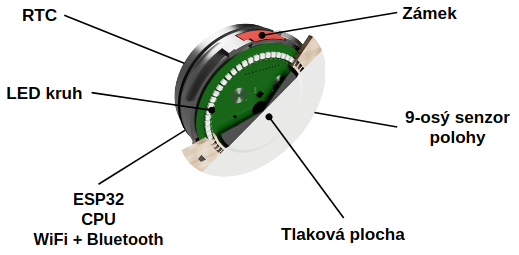
\includegraphics[width=0.95\textwidth]{img/hardware.png}
        \end{center}
        \caption{Hardware}
        \label{fig:hardware}
    \end{small}
\end{figure}

\begin{itemize}[noitemsep]
    \item Hlavní řídící modul
        \begin{itemize}[noitemsep]
            \item ESP32 včetně Wi-fi a bluetooth
            \item Real Time Clock
        \end{itemize}
    \item Uživatelské rozhraní
          \begin{itemize}[noitemsep]
              \item Touchpad
              \item LED kruh
          \end{itemize}
    \item Zámek
        \begin{itemize}[noitemsep]
            \item Motor
            \item Enkodér
            \item IR přijímač
            \item IR vysílač
            \item Zámek sériové linky
        \end{itemize}
    \item Senzory prostředí
          \begin{itemize}[noitemsep]
              \item Magnetometr
              \item Akcelerometr
              \item Gyroskop
              \item Barometr
          \end{itemize}
\end{itemize}

\newpage
\section{Hlavní řídící modul}
Hlavní řídící modul slouží jako výpočetní a~řídící centrum celé desky.

\subsection{ESP32}
BlackBox používá ESP32-WROVER jako svůj procesor.
Základní informace:
\begin{itemize}
    \item Dual core
    \item 240~MHz
    \item 4MB flash
    \item 8MB PSRAM
    \item WiFi, Bluetooth
\end{itemize}

\subsection{Real Time Clock}
Kvůli snížení spotřeby energie bylo implementováno několik mechanismů
Jeden z~těchto mechanismů je i~vypínání všech nepotřebných periferií a~uspání ESP32.V~takovém případě ale není možné uchovat aktuální čas, proto byl na BlackBox přidán modul RTC, ten je napájen přímo z~baterií a~není tak závislý na zbytku BlackBoxu.

\section{Uživatelské rozhraní}

\subsection{Touchpad}
Touchpad je postavený na čipu LDC1614 a jeho alternativách.\footnote{Použitelné jsou pouze alternativy se 4~kanály t.j.~ty, co mají tvar názvu LDCXX14}
Pro měření stisku se využívá deformace kovové destičky a~indukčního měření její vzdálenosti od 4~plošných cívek.
\fxnote{Tady se dá potenciálně napsat spousta věcí :D}

\subsection{LED kruh}
Kruh sestává z~60~adresovatelných RGB LED diod typu WS2812B.

\section{Zámek}

\subsection{Motor a~Encodér}
Zamykací mechanismus je sestaven tak, aby šel BlackBox zasunout do zad trezoru i~v zamčeném stavu, obejde se tedy bez kontroly toho, jestli je při zamykání zasunutý nebo ne.

\subsection{IR komunikace}
IR komunikace je zde obsažená hlavně kvůli synchronizaci se zády trezoru, přesněji k~identifikaci, do kterých zad je BlackBox zasunut.
Tato identifikace by se potenciálně dala dělat pomocí senzorů prostředí, ale za účelem jednoduchosti a~redundance byla zvolena tato možnost.

\subsection{Zámek sériové linky}
Tento mechanismus byl navrhnut za účelem ochrany BlackBox proti neautorizovanému přepsání softwaru.

\section{Senzory prostředí}

\subsection{Senzory polohy}
Tato sada senzorů (akcelerometr, gyroskop, magnetometr) je na různých verzích desky realizována různým způsobem, na verzi 1.0~je realizována jedním čipem obsahujícím všechny tři senzory, ale na verzi 1.1~je realizována pomocí dvou čipů (akcelerometr + gyroskop a~magnetometr)\footnote{Verze 1.1~je zpětně kompatibilní, takže se na ni dá osadit i~čip z~verze 1.0, toho je však v~době psaní této práce nedostatek a~proto byl nahrazen na verzi 1.1 dvěma běžnějšími čipy.}.
Knihovna však musí podporovat všechny možnosti.
Tyto senzory zjišťují natočení BlackBoxu v~prostoru v~9ti osách.
Do budoucna se chystá rozšíření o~GPS senzor.

\subsection{Barometr}
Barometr zde slouží hlavně k hrubému měření výšky, na které se BlackBox nachází.
Případně se také dá použít jako primitivní způsob předpovědi počasí.

\chapter{Technologie}

\section{Framework}

Pro vývoj na microcontroller ESP32 se používájí hlavně dva frameworky a~to ESP-IDF\cite{ESP-IDF} a Arduino\cite{arduino}, oba jsou pro jazyk C/C++.

\subsection{ESP-IDF}

ESP-IDF, nebo také Espressif IoT Development Framework je oficiální framework od výrobce ESP32, firmy Espressif Systems\cite{espressif}.
Je psaný pro vývoj v~jazyce C a~C++, samotný je psaný v~jazyce C.
Obsahuje několik úrovní abstrakce od přímé práce s~registry pro uživatelsky přívětivé API.


\lstinputlisting[language=C++, caption=ESP-IDF]{code/esp-idf.cpp}


\subsection{Arduino}

Arduino je pro začátečníka jednoduší na pochopení a~na práci než ESP-IDF, protože funguje jako úroveň abstrakce nad ESP-IDF.
Jeho obrovskou předností a~zároveň jeho největší limitací je jeho kompatibilita pro množství naprosto rozličných platforem a~architektur sahající až po 8-bitové mikročipy ATtiny.~Bohužel stabilní vývojová větev Arduina pro ESP32 používá zastaralou verzi ESP-IDF, která má některá omezení, kupříkladu nepodporuje C++ 17.

\lstinputlisting[language=C++, caption=Arduino]{code/arduino.cpp}

\subsection{Další frameworky}

Samozřejmě existují i~další frameworky, kupříkladu MicroPython\cite{uPython} a~CircuitPython\cite{circuitPython}, které přivádí jazyk Python na mikrokotrolery, nebo Espruino\cite{espruino}, které dělá to samé pro JavaScript.

\subsection{Výběr}

Pro BlackBox jsem se rozhodl použít přímo ESP-IDF.
K~tomuto rozhodnutí mě vedl fakt, že moje knihovna bude sloužit jako úroveň abstrakce, tudíž Arduino mezivrstva je v~podstatě zbytečná, zároveň tím získám lepší kontrolu nad ESP32.
Protiargumentem by mohlo být množství knihoven dostupných pro Arduino.
Bohužel tyto knihovny nedodržují žádný společný rámec a~většina z~nich není uzpůsobena pro práci na více jádrových procesorech, jakým ESP32 je.\footnote{Nejsou thread safe.}

\section{Použité knihovny}

\begin{itemize}
    \item SmartLeds --
        Knihovna pro interakci s chytrými led WS2812 pomocí hardwarové periferie na ESP32. %todo odkazy, zdroje
    \item Eventpp --
        Knihovna pro jednoduchou práci s událostmi
\end{itemize}

\chapter{Architektura}

BlackBox byl zamýšlen pro tři skupiny uživatelů, přičemž každá má jiné potřeby.
Projekt je rozdělený na tři části, které korespondují se třemi způsoby využití BlackBoxu:

\begin{figure}[h]
    \begin{small}
        \begin{center}
            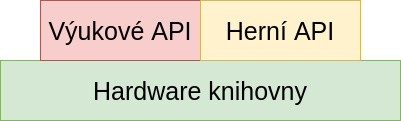
\includegraphics[width=0.95\textwidth]{img/Pyramida2.png}
        \end{center}
        \caption{Tři přístupy}
        \label{fig:Pyramida2}
    \end{small}
\end{figure}

\begin{figure}
    \begin{small}
        \begin{center}
            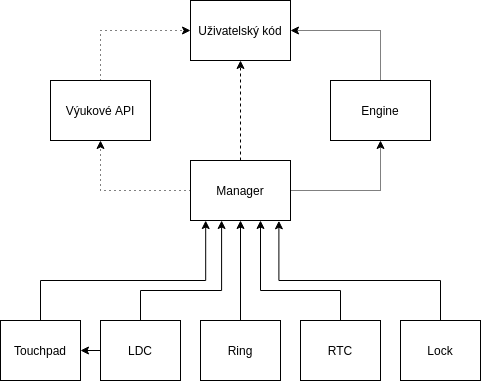
\includegraphics[width=0.95\textwidth]{img/Everything.png}
        \end{center}
        \caption{Graf závislostí}
        \label{fig:everything}
    \end{small}
\end{figure}


% \begin{enumerate}
%     \item Řídící prvky hardwaru
%     \begin{enumerate}
%         \itema~       
%     \end{enumerate}
%     \item Manager hardware prvků

%     Třída určená pro zjednodušenou práci se všemi prvky hardware naráz, aniž by docházelo ke kolizím.
%     \fxnote{popis co to má být}
% \end{enumerate}



\chapter{Výukové API}

Výukové API je navržené pro výuku programování od naprostých začátků, proto musí být co nejjednodušší na pochopení a~použití.
Zároveň by však neměla omezovat využití všech možností knihovny.
Z~toho důvodů používá výukové API pouze jednoduché funkce.
Protože i~použití namespace by mohlo pro začátečníky být složité, nejsou tyto funkce součástí žádného namespace, místo toho pro rozlišení používají prefix "bb" (BlackBox).

\lstinputlisting[language=C++, caption=Výukové API]{code/edu.cpp}

\section{Příklady použití}

Pro výuku programování se BlackBox dá použít dvěma způsoby.

\subsection{Běžná výuka}

Běžnou výukou je myšlena výuka programování tak, jak běžně probíhá na většině škol, pouze místo programování nezajímavé konzolové aplikace budou žáci programovat interaktivní hračku, která na ně může blikat a jinak s~nimi interagovat \footnote{A to případně i onou formou terminálu, uznal by-li to vyučující za vhodné.}, což může výrazně vylepšit motivaci k~učení se programovat.

\subsection{Výuka hrou}

Výuka hrou představuje mix mezi herním a~výukovým API, respektive využívá výukovou (výrazně zjednodušenou) verzi herního API.

Právě pro výuku programování jsem vymyslel hru pro Robotický tábor.
Idea této hry spočívá ve vytvoření sady úloh, v~nichž se BlackBox se základním softwarem chová jako pomůcka pro jejich řešení.

Jednou z úloh může být odemykání virtuálních zámků, kdy BlackBox bude fungovat jako "šperhák".
Na stanovišti budou záda pro BlackBox, do kterých účastník vloží svůj BlackBox, na LED kruhu se budou jeden po druhém objevovat body, kterými musí účastník plynule projet prstem po touchpadu.
Po projetí určitého počtu bodů bude úloha hotova.

Na začátku tábora by si účastnící zahráli tuto hru.
Časová náročnost jednotlivých stanovišť je úmyslně vypočítána tak, aby nebylo možné v~časovém limitu splnit všechna stanoviště, ale aby bylo možné si je všechny vyzkoušet.

Zbytek tábora pak účastníci budou vylepšovat své pomůcky, použijeme-li opět příklad "šperháku", pak ono vylepšení bude sestávat z~automatického řízení "šperháku", namísto fyzického posouvání prstem po touchpadu. Tato pomůcka výrazně urychlí dokončení stanoviště.
Účastníci mají po celou dobu přístup k~jednotlivým stanovištím pro účely testování.

Hra se bude hrát na začátku a na konci tábora, což dává účastníků spoustu času na vylepšování a testování jejich pomůcek.


\chapter{Herní API}
Tato část softwaru je programována za účelem jednoduché tvorby komplexních outdoorových her.
Toho se snaží dosáhnout velkou modulárností a~zaměřením na principy OOP.

\section{Stránky}

Pro vytváření jednoduchých her a~uživatelsky přívětivých menu je implementován systém stránek (Page) a~aplikací (App).

\subsection{Page}

Stránka je soubor barev jednotlivých pozic na displeji (LED kruh) společně s~akcemi při jejich zvolení, nebo při jiné události\footnote{Zatřesení BlackBoxem, povel z případné nadřazené jednotky \dots}.
Prováděné akce jsou uživatelem definované funkce.
Pro pohodlnost je však implementováno několik základních akcí, například blikání.

Speciálním typem předdefinované akce je Link.
Link je způsob propojování více stránek mezi sebou, kupříkladu pokud zvolíte specifickou pozici na první stránce, přehodí vás Link na stránku druhou.\footnote{Toto se dá použít pro tvorbu jednoduchých bludišť.}
Přehození kontextu na jinou stránku je vždy poslední provedená akce vyvolaná událostí.

\subsection{App}

Aplikace je jednoúčelový podprogram zapadající do systému stránek, chová se vlastně jako speciální Page.
Zatímco page je statická (v průběhu kódu se zásadně nemění), aplikace je velmi dynamická.
Do aplikace se dá jednoduše naprogramovat, cokoliv bude uživatel vyžadovat, kupříkladu:
\begin{itemize}
    \item Navigace
    \item Logické hádanky
    \item Hodiny
    \item A~mnoho dalších \dots
\end{itemize}

\section{Zamykání}

Ačkoliv může slovo zamykání na elektronické sejfu, kterým BlackBox je, vyvolat myšlenku o~zamykání tohoto sejfu, není tomu tak.
Funkce zamykání funguje se spoustou věcí.
Primárně však tento systém funguje inhibitor událostí a~přepínání mezi instancemi Page a~Application.

\subsection{Latch}
Latch je zamykací primitivum.
Každý typ Latch má jinou odemykacím/zamykací podmínku.
Mohou být vázané na některý z~senzorů prostředí, Orientation latch lze nastavit, aby k odemknutí vyžadoval otočení BlackBoxu čelem k severu, což zjistí díky zabudovanému magnetometru.

Dalším příkladem může být Time Interval Latch, která se odemkne v~případě, že aktuální čas je v~definovaném rozsahu.

Kromě senzorů však může být Latch ovládán také z~jiných částí kódu, nebo dokonce z~úplně jiného zařízení, k~tomu slouží Remote Latch.

\subsection{Lock}

Lock je třída, která spravuje jednotlivé Latch objekty a~v závislosti na svém typu se odemyká a~zamyká v~závislosti na stavu podřazených Latch.
Mezi tyto typy patří například:
\begin{itemize}
    \item All -- AND
    \item None -- NAND
    \item AtLeast(n) -- alespoň n Latch musí být odemkneno
    \item Weighted(x) -- Každé latch je přiřazena váha, součet vah odemknených Latch potom musí být >= x
    \item A~další \dots
\end{itemize}
Lock také může být vložen do dalšího Lock objektu.

\begin{figure}[H]
    \begin{small}
        \begin{center}
            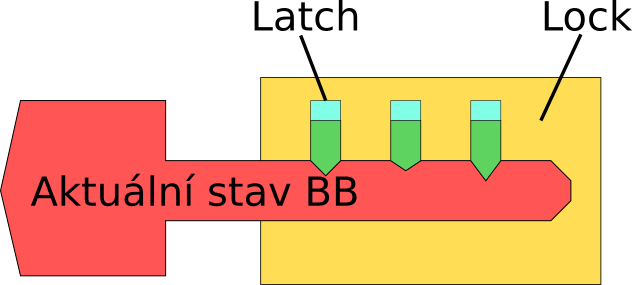
\includegraphics[width=0.95\textwidth]{img/lock.png}
        \end{center}
        \caption{Idea zámku}
        \label{fig:lock}
    \end{small}
\end{figure}

\newpage

\section{Příklady použití}

\lstinputlisting[language=C++, caption=Ukázka propojování stránek]{code/pageSimple.cpp}

\begin{figure}[H]
    \begin{small}
        \begin{center}
            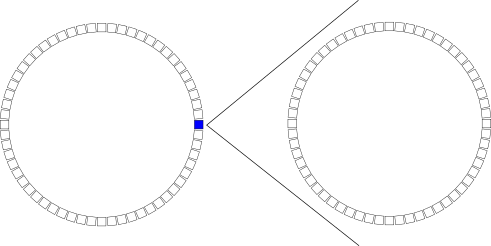
\includegraphics[width=0.95\textwidth]{img/pageLink.png}
        \end{center}
        \caption{Vizualizace výsledku ukázky propojování stránek}
        \label{fig:pageLink}
    \end{small}
\end{figure}

\newpage

\lstinputlisting[language=C++, caption=Ukázka propojování aplikací]{code/appSimple.cpp}

\begin{figure}[H]
    \begin{small}
        \begin{center}
            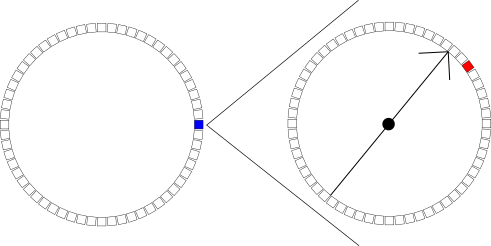
\includegraphics[width=0.95\textwidth]{img/appLink.png}
        \end{center}
        \caption{Vizualizace výsledku ukázky propojování aplikací}
        \label{fig:appLink}
    \end{small}
\end{figure}

\newpage

\lstinputlisting[language=C++, caption=Ukázka práce s herním API]{code/page.cpp}

\newpage

Pro potřeby této práce je \textbf{synchronní hra} taková hra k~jejímuž hraní je potřeba interakce hráčů v~reálném čase ať už s~"prostředím", nebo mezi sebou.
\textbf{Asynchronní} je poté hra, která nevyžaduje interakce v~reálném čase.

\subsection{Synchronní hry}

\subsubsection{Lights out/Večerka}

Hraje se v~noci s~BlackBoxy rozmístěnými v~mřížce na louce, část BlackBoxů svítí a~část ne.
Při zmáčknutí BlackBoxu se změní stav daného BlackBoxu spolu se stavy okolních BlackBoxů podle předem daného pravidla.
Cílem je vypnout všechny světla.

\subsubsection{Path of light/Světelná cesta}

Pro efekt je lepší hrát tuto hru v~noci.
Každý hráč má svůj BlackBox.
V~prostoru jsou rozmístěny zad pro BlackBox v~předem daných polohách.
V~závislosti na věku hráčů, herním čase a~dostupné prostoru může být herní plocha rozlehlá i~několik set metrů.
Je několik počátečních pozic.

Každý hráč má vygenerované bludiště, kde cesty jsou definované jako spojnice mezi BlackBoxy (toto bludiště se může autonomně měnit v~průběhu hry).
Když hráč dojde na stanoviště a~zasune svůj BlackBox do zad na stanovišti, zobrazí se mu možné směry, kterými se může vydat.
Hráč si jeden z~nich vybere a~BlackBox mu začne ukazovat přímou spojnici ke stanovišti v~daném směru.
Pokud hráč sejde z~originální přímé spojnice, může si opravit směr na jakémkoliv dalším stanovišti.

Hráč vyhrává, pokud se dostane do středu bludiště.


\subsection{Asynchronní hry}

Typickým příkladem asynchronní hry jsou šifrovací hry, kdy hráči dostanou na vyluštění delší časový úsek, hra potom může být rozdělena na etapy.
Začátek etapy bude sloužit jako synchronizační a~vylučovací bod.
Tento způsob šifrovací hry snižuje potřebu koordinace, protože ji každý může řešit "až bude mít čas."


\chapter{Hardwarové knihovny}
Hardwarové knihovny jsou nejnižší částí BlackBoxu.
Každá knihovna obsluhuje nějakou periferii a slouží k interakci s ní.
Hardwarové knihovny jsou rozdělené\footnote{Pouze v tomto textu, v kódu toto rozdělení není.} do několika částí:

\section{Hlavní řídící modul}

Součástí hlavního modulu je samotný řídící čip ESP32 a RTC.

\subsection{RTC}\label{ss:rtc}

RTC slouží k uchování času při šetření baterie tím, že umožňuje uspání zbytku BlackBoxu.
Stejně jako ostatní I$^2$C periferie\footnote{T.j. RTC, LDC, barometr, senzory polohy.} používá RTC virtuální dvojče, tzn. že v programu existuje kopie všech registrů, běžný uživatel pak pracuje pouze s touto kopií, která se periodicky synchronizuje a provádí přitom kontrolu nastavovaných hodnot.
Toto urychluje kontrolu nastavovacích registrů a zároveň zjednodušuje potenciální tvorbu simulátoru.
Pokročilejší uživatelé mohou pracovat přímo s jednotlivými registry a dvojče používat pouze na rychlou kontrolu hodnot.

\section{Uživatelské rozhraní}

Uživatelské rozhraní je pro běžného uživatele asi nejužitečnější části knihovny, protože slouží právě k interakci s ním.

\subsection{Touchpad}

Třída Touchpad slouží jako most mezi uživatelem a třídou LDC.
Je zodpovědná za přepočet surových dat z LDC do souřadnic doteku a jeho síly.

\begin{figure}[H]
    \begin{small}
        \begin{center}
            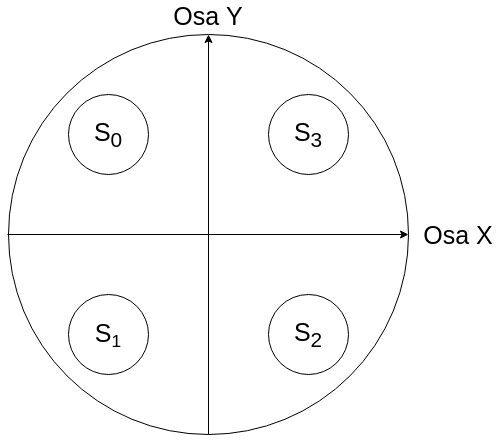
\includegraphics[width=0.95\textwidth]{img/Touchpad_calculation.png}
        \end{center}
        \caption{Výpočet pozice doteku}
        \label{fig:touchpad_calculation}
    \end{small}
\end{figure}

\begin{listedequation}[H]
    \begin{center}
        $X = -k_0S_0 -k_1S_1 +k_2S_2 +k_3S_3$\\
        $Y = +k_0S_0 -k_1S_1 -k_2S_2 +k_3S_3$\\
        $Tlak = \frac{k_0S_0 +k_1S_1 +k_2S_2 +k_3S_3}{4}$
    \end{center}
    \caption{Výpočet parametrů doteku}
    \label{eq:touchpad_calculation_X}
\end{listedequation}

\subsubsection{LDC}

Třída LDC se stará o komunikaci s čipem LDC1614.
Sama nedělá žádné výpočty, dělá pouze základní filtraci dat.
Jedná se o I$^2$C senzor\footnote{Používá virtuální dvojče. \autoref{ss:rtc}.}.

\subsection{LED kruh}

% ? Should I write about 2.0?
LED kruh poskytuje kromě příjemného subscript operátoru pro přístup k jednotlivým LED také možnost vykresloval celé obrazce (kružnice a oblouky).
Umožňuje také nastavit maximální hodnotu displeje, všechny barvy jsou poté vyškálovány do tohoto rozsahu.
Za použití akcelerometru je také možné displej převracet v závislosti na jeho natočení, jak je zvykem u mobilních telefonů.

LED kruh je postaven na knihovně SmartLeds\cite{SmartLeds}.

\section{Zámek}

Tato sekce je důležitá především, pokud budete chtít používat Blackbox jako elektronický sejf.

\subsection{Lock}

Lock spravuje motor a magnetický enkodér.
Ty dohromady tvoří zámek, který je schopen poznat, v jakém stavu se nachází, bez nutnosti tuto informaci udržovat v paměti.
Důležitý je fakt, že zámek je designovaný tak, aby se BlackBox dal vložit do protikusu, aniž by bylo nutné jej odemykat.

\subsection{IR komunikace}

IR komunikace je určená k jednoduché komunikaci mezi BlackBox a Chytrými zády\footnote{Protikus BlackBoxu s vlastní elektronikou.}.


\section{Senzory prostředí}

\subsection{Senzory polohy}

Množství funkcionality poskytuje BlackBoxu možnost detekovat natočení v 9 osách. %todo tady toho asi dost chybí? 

\section{Příklady použití}

Hardwarové knihovny mají asi nejširší možnosti použití.
Dvěma z nich mohou být i herní a výukové API.

Knihovny se nemusí používat pouze v rámci desky BlackBox, ale také mimo ni jako samostatné knihovny.
Kupříkladu LED kruh se dá použít na řízení jakéhokoliv displeje, který má imitovat ručičkové ukazatele.
Touchpad může být sám o sobě také velmi užitečný.


\chapter{Dokumentace}

Ke všem částem knihovny je dostupná česko-anglická dokumentace.

Dokumentace je dostupná online\cite{dokumentace}.

% \fxfatal{Víc!}

\chapter{Závěr}

Vytvořil jsem sadu knihoven pro práci s deskou BlackBox zaměřenou na vývoj her a výuku programování.
Tato knihovna je jednoduchá na použití a přitom poskytuje širokou škálu možností.
Na této knihovně byla ve školním roce 2019/20 vedena část kroužku, bohužel tento kroužek nemohl být dokončen kvůli globální pandemii.
Kvůli pandemii také nebylo zatím možné použít BlackBox na žádné šifrovací hře, vzhledem k nemožnosti jejich konání.

V práci na BlackBox budu i na dále pokračovat a to nejen na rozšířování o periferie chystané pro verzi 2.0 hardwarové desky, která bude přidávat hlavně GPS, GPRS a sekundární procesor.
Ale také vytvářením pomůcek jako například grafický editor a generátor her.

Tato knihovna je dostupná jako zdrojový kód\cite{BlackBox-software}, ale také i jako knihovna v PlatformIO registry\cite{pio-registry}.

\newpage
\printbibliography[title=Literatura]
\addcontentsline{toc}{section}{Literatura}

\listoffigures
\addcontentsline{toc}{section}{Seznam obrázků}

\listoftables
\addcontentsline{toc}{section}{Seznam tabulek}

\listoflistedequation
\addcontentsline{toc}{section}{Seznam rovnic}

\lstlistoflistings
\addcontentsline{toc}{section}{\lstlistlistingname}

\end{document}
